\documentclass{standalone}
\usepackage{tikz}
\usetikzlibrary{calc}
\begin{document}
    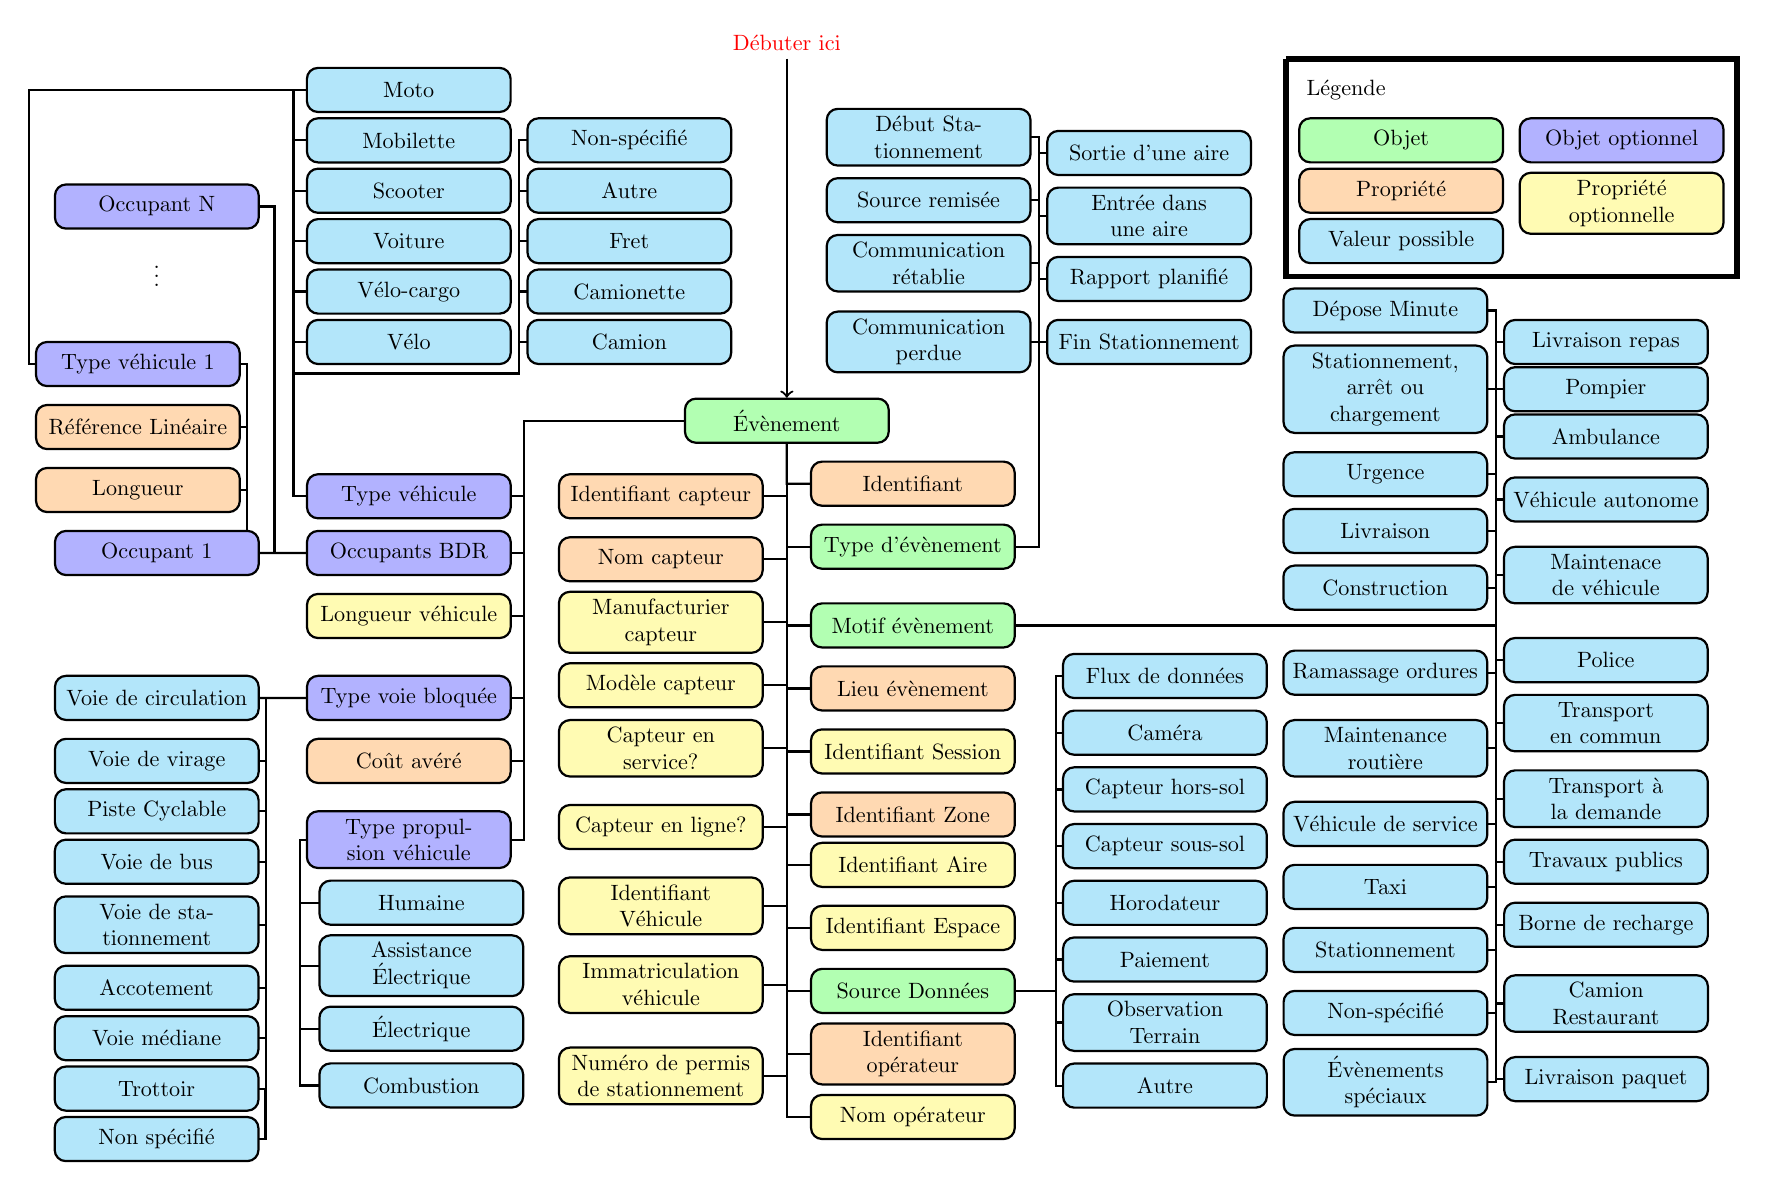
\begin{tikzpicture}[thick,scale=0.8, every node/.style={scale=0.8}]
        \tikzstyle {objet} = [rectangle, rounded corners, text width=3cm, minimum height=0.7cm,text centered,  draw=black, fill=green!30]
        \tikzstyle {objet_opt} = [rectangle, rounded corners, text width=3cm, minimum height=0.7cm,text centered,  draw=black, fill=blue!30]
        \tikzstyle {propriete} = [rectangle, rounded corners, text width=3cm, minimum height=0.7cm,text centered,  draw=black, fill=orange!30]
        \tikzstyle{propriete_opt} =[rectangle, rounded corners, text width=3cm, minimum height=0.7cm,text centered,  draw=black, fill=yellow!30]
        \tikzstyle{enumeration} = [rectangle, rounded corners, text width=3cm, minimum height=0.7cm,text centered,  draw=black, fill=cyan!30]
        \node (event) [objet]{Évènement};
        \node (debut)[color=red,above of=event,yshift=5cm]{Débuter ici};
        \draw [->] (debut.south) -- (event.north);
        \node (id) [propriete,below of=event,xshift=2cm]{Identifiant};
        % type et enumeration
        \node (type) [objet, below of=id]{Type d'évènement};
        \node (comms_perdues) [enumeration, right of=type,xshift=-0.75cm,yshift=3.25cm]{Communication perdue};
        \node (comms_retablies)[enumeration, above of=comms_perdues,yshift=0.25cm]{Communication rétablie};
        \node (remise) [enumeration, above of=comms_retablies]{Source remisée};
        \node (park_start) [enumeration, above of=remise]{Début Stationnement};
        \node (park_end) [enumeration, right of=comms_perdues,xshift=2.5cm]{Fin Stationnement};
        \node (rapport_planifie) [enumeration, above of=park_end]{Rapport planifié};
        \node (enter_area) [enumeration, above of=rapport_planifie]{Entrée dans une aire};
        \node (exit_area) [enumeration, above of=enter_area]{Sortie d'une aire};
        \coordinate (type_enum_centre) at ($(comms_perdues)!0.5!(park_end)$);
        \draw (type) -| (type_enum_centre) |- (comms_perdues);
        \draw (comms_perdues) -| (type_enum_centre) |- (park_end);
        \draw (comms_perdues) -| (type_enum_centre) |- (rapport_planifie);
        \draw (rapport_planifie) -| ($(rapport_planifie -| type_enum_centre)$) |- (comms_retablies);
        \draw (comms_retablies) -| ($(comms_retablies -| type_enum_centre)$) |- (enter_area);
        \draw (enter_area) -| ($(enter_area -|type_enum_centre)$) |- (remise);
        \draw (remise) -| ($(remise -| type_enum_centre)$) |- (exit_area);
        \draw (exit_area) -| ($(exit_area -| type_enum_centre)$) |- (park_start);
        % Motif et /num/ration
        \node (purpose) [objet, below of=type,yshift=-0.25cm]{Motif évènement};
        \node (construction) [enumeration] at ($(purpose) + (7.5,0.6)$){Construction};
        \node (livraison) [enumeration, above of=construction,yshift=-0.1cm]{Livraison};
        \node (urgence) [enumeration,above of=livraison,yshift=-0.1cm]{Urgence};
        \node (parking) [enumeration, above of=urgence,yshift=0.35cm]{Stationnement, arrêt ou chargement};
        \node (passenger_transport) [enumeration,above of=parking,yshift=0.25cm]{Dépose Minute};
        
        \node (waste_man) [enumeration] at ($(purpose -| construction) +(0,-0.75)$){Ramassage ordures};
        \node (maintenance_routier) [enumeration, below of=waste_man,yshift=-0.2cm]{Maintenance routière};
        \node (service_veh)[enumeration,below of=maintenance_routier,yshift=-0.2cm]{Véhicule de service};
        \node (taxi) [enumeration,below of=service_veh]{Taxi};
        \node (stationnement) [enumeration, below of=taxi]{Stationnement};
        \node (autre) [enumeration, below of=stationnement]{Non-spécifié};
        \node (evenement_special) [enumeration, below of=autre,yshift=-0.1cm]{Évènements spéciaux};
        
        \node (device_main) [enumeration,right of=construction,xshift=2.5cm,yshift=0.2cm]{Maintenace de véhicule};
        \node (autonomous) [enumeration, above of=device_main,yshift=0.2cm]{Véhicule autonome};
        \node (ems) [enumeration, above of=autonomous]{Ambulance};
        \node (fire) [enumeration, above of=ems,yshift=-0.25cm]{Pompier};
        \node (food_deliv)[enumeration, above of=fire,yshift=-0.25cm]{Livraison repas};
        
        \node (police) [enumeration,right of=waste_man,xshift=2.5cm,yshift=0.2cm]{Police};
        \node (TC) [enumeration,below of=police]{Transport en commun};
        \node (transport_demande) [enumeration, below of=TC,yshift=-0.2cm]{Transport à la demande};
        \node (utility_work)[enumeration, below of=transport_demande]{Travaux publics};
        \node (chargement) [enumeration, below of=utility_work]{Borne de recharge};
        \node (vente) [enumeration, below of=chargement,yshift=-0.25cm]{Camion Restaurant};
        \node (parcel_deliv) [enumeration, below of=vente,yshift=-0.2cm]{Livraison paquet};
        \coordinate (center_point_motif) at ($(construction)!0.5!(police)$);
        \draw (purpose) -| (center_point_motif) |- (construction);
        \draw (construction) -|(center_point_motif) |-(police);
        \draw (construction) -| ($(construction -| center_point_motif)$) |-(device_main);
        \draw (device_main) -| ($(device_main -| center_point_motif)$) |-(livraison);
        \draw (livraison) -| ($(livraison -| center_point_motif)$) |- (autonomous.west);
        \draw (autonomous) -| ($(autonomous -|center_point_motif)$) |- (urgence.east);
        \draw (urgence) -| ($(urgence -| center_point_motif)$) |- (ems); 
        \draw (ems) -| ($(ems -| center_point_motif)$) |- (parking);
        \draw (parking) -| ($(parking -| center_point_motif)$) |- (fire);
        \draw (fire) -| ($(fire -| center_point_motif)$) |- (food_deliv);
        \draw (passenger_transport) -| ($(food_deliv -| center_point_motif)$ |- (food_deliv);
        \draw (passenger_transport) -| ($(passenger_transport -| center_point_motif)$) |- (parcel_deliv);
        \draw (parcel_deliv) -| ($(parcel_deliv -| center_point_motif)$) |- (evenement_special);
        \draw (police) -| ($(police-|center_point_motif)$) |- (waste_man);
        \draw (waste_man) -| ($(waste_man-|center_point_motif)$) |- (TC);
        \draw (TC) -| ($(TC-|center_point_motif)$) |- (maintenance_routier);
        \draw (maintenance_routier) -| ($(maintenance_routier-|center_point_motif)$) |- (transport_demande);
        \draw (transport_demande) -| ($(transport_demande-|center_point_motif)$) |- (service_veh);
        \draw (service_veh) -| ($(service_veh-|center_point_motif)$) |- (utility_work);
        \draw (utility_work) -| ($(utility_work-|center_point_motif)$) |- (taxi);
        \draw (taxi) -| ($(taxi-|center_point_motif)$) |- (chargement);
        \draw (chargement) -| ($(chargement-|center_point_motif)$) |- (stationnement);
        \draw (stationnement) -| ($(stationnement-|center_point_motif)$) |- (vente);
        \draw (vente) -| ($(vente-|center_point_motif)$) |- (autre);
        
        % LIeu
        \node (lieu) [propriete, below of=purpose]{Lieu évènement};
        \node (id_session) [propriete_opt,below of=lieu]{Identifiant Session};
        \node (id_zone) [propriete, below of=id_session]{Identifiant Zone};
        \node (id_aire) [propriete_opt, below of=id_zone,yshift=0.2cm]{Identifiant Aire};
        \node (id_espace) [propriete_opt, below of=id_aire]{Identifiant Espace};
        % Sources de données
        \node (source_donnee) [objet, below of=id_espace]{Source Données};
        \node (flux_donnees) [enumeration, right of=source_donnee,xshift=3cm,yshift=5cm]{Flux de données};
        \node (camera) [enumeration,below of=flux_donnees,yshift=0.1cm]{Caméra};
        \node (above_ground) [enumeration, below of=camera,yshift=0.1cm]{Capteur hors-sol};
        \node (in_ground) [enumeration, below of=above_ground,yshift=0.1cm]{Capteur sous-sol};
        \node (meter) [enumeration, below of=in_ground,yshift=0.1cm]{Horodateur};
        \node (paiement) [enumeration, below of=meter,yshift=0.1cm]{Paiement};
        \node (in_person) [enumeration, below of=paiement]{Observation Terrain};
        \node (autre_obs) [enumeration, below of=in_person]{Autre};
        \draw (flux_donnees.west) -| ++(-.1,-.1) |- (camera);
        \draw (camera.west) -| ++(-.1,-.1) |- (above_ground);
        \draw (above_ground.west) -| ++(-.1,-.1) |- (in_ground);
        \draw (in_ground.west) -| ++(-.1,-.1) |- (meter);
        \draw (meter.west) -| ++(-.1,-.1) |- (paiement);
        \draw (paiement.west) -|++(-.1,-.1) |- (source_donnee);
        \draw (in_person.west) -| ++(-.1,-.1)|-(source_donnee);
        \draw (in_person.west)-| ++(-.1,-.1)|- (autre_obs);
        % Fin Source de données
        \node (operator) [propriete, below of=source_donnee]{Identifiant opérateur};
        \node (nom_operateur) [propriete_opt, below of=operator]{Nom opérateur};
        \node (identifiant_capteur) [propriete, below of=event,xshift=-2cm,yshift=-0.2cm]{Identifiant capteur};
        \node (nom_capteur) [propriete, below of=identifiant_capteur]{Nom capteur};
        \node (manufacturier_capteur) [propriete_opt, below of=nom_capteur]{Manufacturier capteur};
        \node (modele_capteur) [propriete_opt, below of=manufacturier_capteur]{Modèle capteur};
        \node (capteur_actif) [propriete_opt, below of=modele_capteur]{Capteur en service?};
        \node (capteur_en_ligne) [propriete_opt,below of=capteur_actif,yshift=-0.25cm]{Capteur en ligne?};
        \node (id_vehicule) [propriete_opt, below of=capteur_en_ligne,yshift=-0.25cm]{Identifiant Véhicule};
        \node (plaque_vehicule) [propriete_opt, below of=id_vehicule,yshift=-0.25cm]{Immatriculation véhicule};
        \node (numero_permis_vehicule) [propriete_opt, below of=plaque_vehicule,yshift=-0.45cm]{Numéro de permis de stationnement};
        % Type véhicule
        \node (type_vehicule) [objet_opt,left of=identifiant_capteur,xshift=-3cm]{Type véhicule};
        \node (velo) [enumeration] at ($ (comms_perdues-|type_vehicule)$) {Vélo};
        \node (velo-cargo) [enumeration, above of=velo,yshift=-0.2cm]{Vélo-cargo};
        \node (char) [enumeration, above of=velo-cargo,yshift=-0.2cm]{Voiture};
        \node (scooter) [enumeration, above of=char,yshift=-0.2cm]{Scooter};
        \node (mobilette) [enumeration, above of=scooter,yshift=-0.2cm]{Mobilette};
        \node (moto) [enumeration, above of=mobilette,yshift=-0.2cm]{Moto};
        \node (camion) [enumeration, right of=velo,xshift=2.5cm]{Camion};
        \node (camionette) [enumeration, above of=camion,yshift=-0.2cm]{Camionette};
        \node (fret) [enumeration, above of=camionette,yshift=-0.2cm]{Fret};
        \node (autre) [enumeration, above of=fret,yshift=-0.2cm]{Autre};
        \node (non-spec-veh) [enumeration, above of=autre,yshift=-0.2cm]{Non-spécifié};
        \coordinate (centre_type_veh) at ($(velo)!0.5!(camion) + (0,-0.5)$);
        \draw (type_vehicule.west) -| ++(-0.2,0.2) |- (velo.west); 
        \draw (velo.west) -| ++(-0.2,0.2) |- (velo-cargo.west);
        \draw (velo-cargo.west) -| ++(-0.2,0.2) |- (char.west);
        \draw (char.west) -| ++(-0.2,0.2) |- (scooter.west);
        \draw (scooter.west) -| ++(-0.2,0.2) |- (mobilette.west);
        \draw (mobilette.west) -| ++(-0.2,0.2) |- (moto.west);
        \draw (type_vehicule.west) -| ++(-0.2,0.2) |- (centre_type_veh) |- (camion.west);
        \draw (camion.west) -| ($(camion -| centre_type_veh)$) |- (camionette.west);
        \draw (camionette.west) -| ($(camionette -| centre_type_veh)$) |- (fret.west);
        \draw (fret.west) -| ($(fret-| centre_type_veh)$) |- (autre.west);
        \draw (autre.west) -| ($(autre-| centre_type_veh)$) |- (non-spec-veh.west);
        % Occupants
        \node (occupants_bdr) [objet_opt, below of=type_vehicule,yshift=0.1cm] {Occupants BDR};
        \node (occupant_bdr) [objet_opt, left of=occupants_bdr,xshift=-3cm] {Occupant 1};
        \node (longueur_occupant_1) [propriete, above of=occupant_bdr,xshift=-0.3cm]{Longueur};
        \node (reference_lineaire_1) [propriete, above of=longueur_occupant_1]{Référence Linéaire};
        \node (type_occupant_1) [objet_opt,above of=reference_lineaire_1]{Type véhicule 1};
        \draw (longueur_occupant_1.east) -| ++(0.1,-0.1) |- ($(occupant_bdr.north-|longueur_occupant_1.east)+(0.1,0)$);
        \draw (reference_lineaire_1.east)-| ++(0.1,-0.1) |- (longueur_occupant_1.east);
        \draw (type_occupant_1.east)-| ++(0.1,-0.1) |- (reference_lineaire_1.east);
        \draw (type_occupant_1.west) -| ++(-0.1,0.1) |- (moto.west);
        \node (occupant_bdr_n) [objet_opt, above of=occupant_bdr,yshift=4.5cm]{Occupant N};
        \node (dots) [below of=occupant_bdr_n]{\vdots};
        \draw (occupants_bdr.west) --(occupant_bdr.east);
        \draw (occupants_bdr.west) -| ++(-0.5,0.1) |-(occupant_bdr_n.east);
        \node (longueur_vehicule) [propriete_opt, below of=occupants_bdr]{Longueur véhicule};
        % Type voie
        \node (type_voie_bloquee) [objet_opt, below of=longueur_vehicule,yshift=-0.3cm] {Type voie bloquée};
        \node (voie_transit) [enumeration, left of=type_voie_bloquee,xshift=-3cm]{Voie de circulation};
        \node (voie_virage) [enumeration, below of= voie_transit]{Voie de virage};
        \node (piste_cyclable) [enumeration, below of=voie_virage,yshift=0.2cm]{Piste Cyclable};
        \node (voie_bus) [enumeration, below of=piste_cyclable,yshift=0.2cm]{Voie de bus};
        \node (voie_stationnement) [enumeration, below of=voie_bus]{Voie de stationnement};
        \node (accotement) [enumeration, below of=voie_stationnement]{Accotement};
        \node (voie_mediane) [enumeration, below of=accotement,yshift=0.2cm]{Voie médiane};
        \node (trottoir) [enumeration , below of=voie_mediane,yshift=0.2cm]{Trottoir};
        \node (voie-non-spec) [enumeration, below of=trottoir,yshift=0.2cm]{Non spécifié};
        \draw (voie-non-spec.east) -| ++(0.1,0.1) |- (trottoir.east);
        \draw (trottoir.east) -|  ++(0.1,0.1) |- (voie_mediane.east);
        \draw (voie_mediane.east) -|  ++(0.1,0.1) |- (accotement.east);
        \draw (voie_stationnement.east) -| ++(0.1,0.1) |- (accotement.east);
        \draw (voie_stationnement.east) -| ++(0.1,0.1) |- (voie_bus.east);
        \draw (voie_bus.east)  -| ++(0.1,0.1) |- (piste_cyclable.east);
        \draw (piste_cyclable.east)  -| ++(0.1,0.1) |- (voie_virage.east);
        \draw (voie_virage.east)  -| ++(0.1,0.1) |- (voie_transit.east);
        \draw (voie_transit.east) -- (type_voie_bloquee.west);
        % cout
        \node (cout_avere) [propriete, below of=type_voie_bloquee] {Coût avéré};
        % Type propulsion
        \node (type_propulsion) [objet_opt, below of=cout_avere,yshift=-0.25cm]{Type propulsion véhicule};
        \node (prop_humaine) [enumeration, below of=type_propulsion,xshift=0.2cm]{Humaine};
        \node (prop_elec_assist) [enumeration, below of=prop_humaine]{Assistance Électrique};
        \node (prop_elec) [enumeration, below of=prop_elec_assist]{Électrique};
        \node (prop_comb) [enumeration, below of=prop_elec,yshift=0.1cm]{Combustion};
        \draw (type_propulsion.west)  -| ++(-0.1,-0.1) |- (prop_humaine.west);
        \draw (type_propulsion.west)  -| ++(-0.1,-0.1) |- (prop_elec_assist.west);
        \draw (type_propulsion.west)  -| ++(-0.1,-0.1) |- (prop_elec.west);
        \draw (type_propulsion.west)  -| ++(-0.1,-0.1) |- (prop_comb.west);
        % evenement
        \draw (type_vehicule.east) -| ++(0.2,0.2) |- (event.west);
        \draw (type_vehicule.east) -| ++(0.2,0.2) |- (occupants_bdr.east);
        \draw (longueur_vehicule.east) -| ++(0.2,0.2) |- (occupants_bdr.east);
        \draw (type_voie_bloquee.east) -| ++(0.2,0.2) |- (longueur_vehicule.east);
        \draw (cout_avere.east) -| ++(0.2,0.2) |- (type_voie_bloquee.east);
        \draw (type_voie_bloquee.east) -| ++(0.2,0.2) |- (type_propulsion.east);
        \coordinate (centre_evenement) at ($(event |-id)$);
        \draw (event.south) --(centre_evenement) -- (id);
        \draw (id.west) -| ($(centre_evenement|-identifiant_capteur)$) |-(identifiant_capteur);
        \draw (identifiant_capteur) -| ($(centre_evenement|-type)$) |-(type);
        \draw (type) -| ($(type -| centre_evenement)$) |- (nom_capteur);
        \draw (nom_capteur) -| ($(nom_capteur -| centre_evenement)$) |- (purpose);
        \draw (purpose) -| ($(purpose -| centre_evenement)$) |- (manufacturier_capteur);
        \draw (lieu) -| ($(lieu -| centre_evenement)$)|- (manufacturier_capteur);
        \draw (modele_capteur) -| ($(modele_capteur -| centre_evenement)$) |- (id_session);
        \draw (id_session) -| ($(id_session -| centre_evenement)$) |-(capteur_actif);
        \draw (capteur_actif) -| ($(capteur_actif -| centre_evenement)$) |- (id_zone);
        \draw (id_zone) -| ($(id_zone -| centre_evenement)$) |-(capteur_en_ligne);
        \draw (capteur_en_ligne) -| ($(capteur_en_ligne -| centre_evenement)$) |- (id_aire);
        \draw (id_aire) -| ($(id_aire-| centre_evenement)$)|- (id_vehicule);
        \draw (id_vehicule) -| ($(id_vehicule -|centre_evenement)$) |- (id_espace);
        \draw (id_espace) -| ($(id_espace -| centre_evenement)$) |- (plaque_vehicule);
        \draw (plaque_vehicule) -| ($(plaque_vehicule -| centre_evenement)$) |- (source_donnee);
        \draw (source_donnee) -| ($(source_donnee -| centre_evenement)$) |- (operator);
        \draw (operator) -| ($(operator -| centre_evenement)$) |- (numero_permis_vehicule);
        \draw (numero_permis_vehicule) -| ($(numero_permis_vehicule -| centre_evenement)$) |- (nom_operateur);
        \node (legend) [text width =3cm,right of=park_start, xshift=6.5cm,yshift=0.75cm]{Légende};
        \node (obj_leg) [objet, below of=legend,yshift=0.2cm]{Objet};
        \node (prop_leg) [propriete, below of=obj_leg,yshift=0.2cm]{Propriété};
        \node (enum_leg) [enumeration , below of=prop_leg,yshift=0.2cm]{Valeur possible};
        \node (obj_opt_leg) [objet_opt, right of=obj_leg,xshift=2.5cm]{Objet optionnel};
        \node (propriete_opt_leg) [propriete_opt, below of=obj_opt_leg]{Propriété optionnelle};
        \coordinate (legend_box_top_left) at ($(legend.north west) + (-0.2,0.2)$);
        \coordinate (legend_box_bottom_right) at ($(enum_leg.south -| propriete_opt_leg.east) + (0.2,-0.2)$);
        \draw[line width=2pt] (legend_box_top_left) -| (legend_box_bottom_right) -| (legend_box_top_left);
    \end{tikzpicture}
\end{document}